\chapter{Theoretical framework}
\label{ch:theory}

This chapter gives an outline of the theoretical concepts and models used in this thesis. It is split into two parts: First, the Standard Model of elementary particle physics is discussed, with an emphasis on the top quark. Secondly, several hypothesized extensions of the Standard Model, relevant for the searches presented in \cref{ch:ah,ch:alps}, are briefly introduced and compared.

\section{Standard Model}

% content:
% particles, interactions, alphaEW, alphas
% top quark: mass, width, lifetime; decay into Wb;
% Yukawa coupling to Higgs, spin analyzing power
% Higgs mechanism: Higgs doublet in the SM, symmetry breaking, result: massive scalar particle; mass, coupling to massive particles
% pp -> ttbar: production diagrams (tree level), production modes (gg / qq), decays: allhad, semilep, dilep; mtt spectrum (?); spin states of ttbar
% spin density matrix: decomposition into polarizations and correlations, linear observables; cite new measurements
% nonperturbative: resummations close to the threshold, Couloumb resummation --> sorta bound state; comparison with J/Psi and Upsilon (large top width), difficulty of modeling: singlet v octet, Fuks model: singlet only, effective model, hints for observation in entanglement paper

The Standard Model of elementary particle physics, often simply called the Standard Model or SM, is, at the time of writing, the most successful theory describing the fundamental particles making up our universe~\cite{Martin:2008zz,Schwartz:2014sze}. It is the result of a steady progression of increasingly complex models, starting with the introduction of quantum mechanics in the early 20th century and ending - for now - with the discovery of the Higgs boson at the LHC in 2012. The model has been extensively tested at many different experiments, most importantly the large collider experiments like PETRA, LEP, HERA, the Tevatron, and the LHC. So far, it has survived most of these tests with excellence, the biggest exception being the observation of neutrino masses (cf. \cref{sec:theory:bsm}).

\begin{figure}[ht]
    \centering
    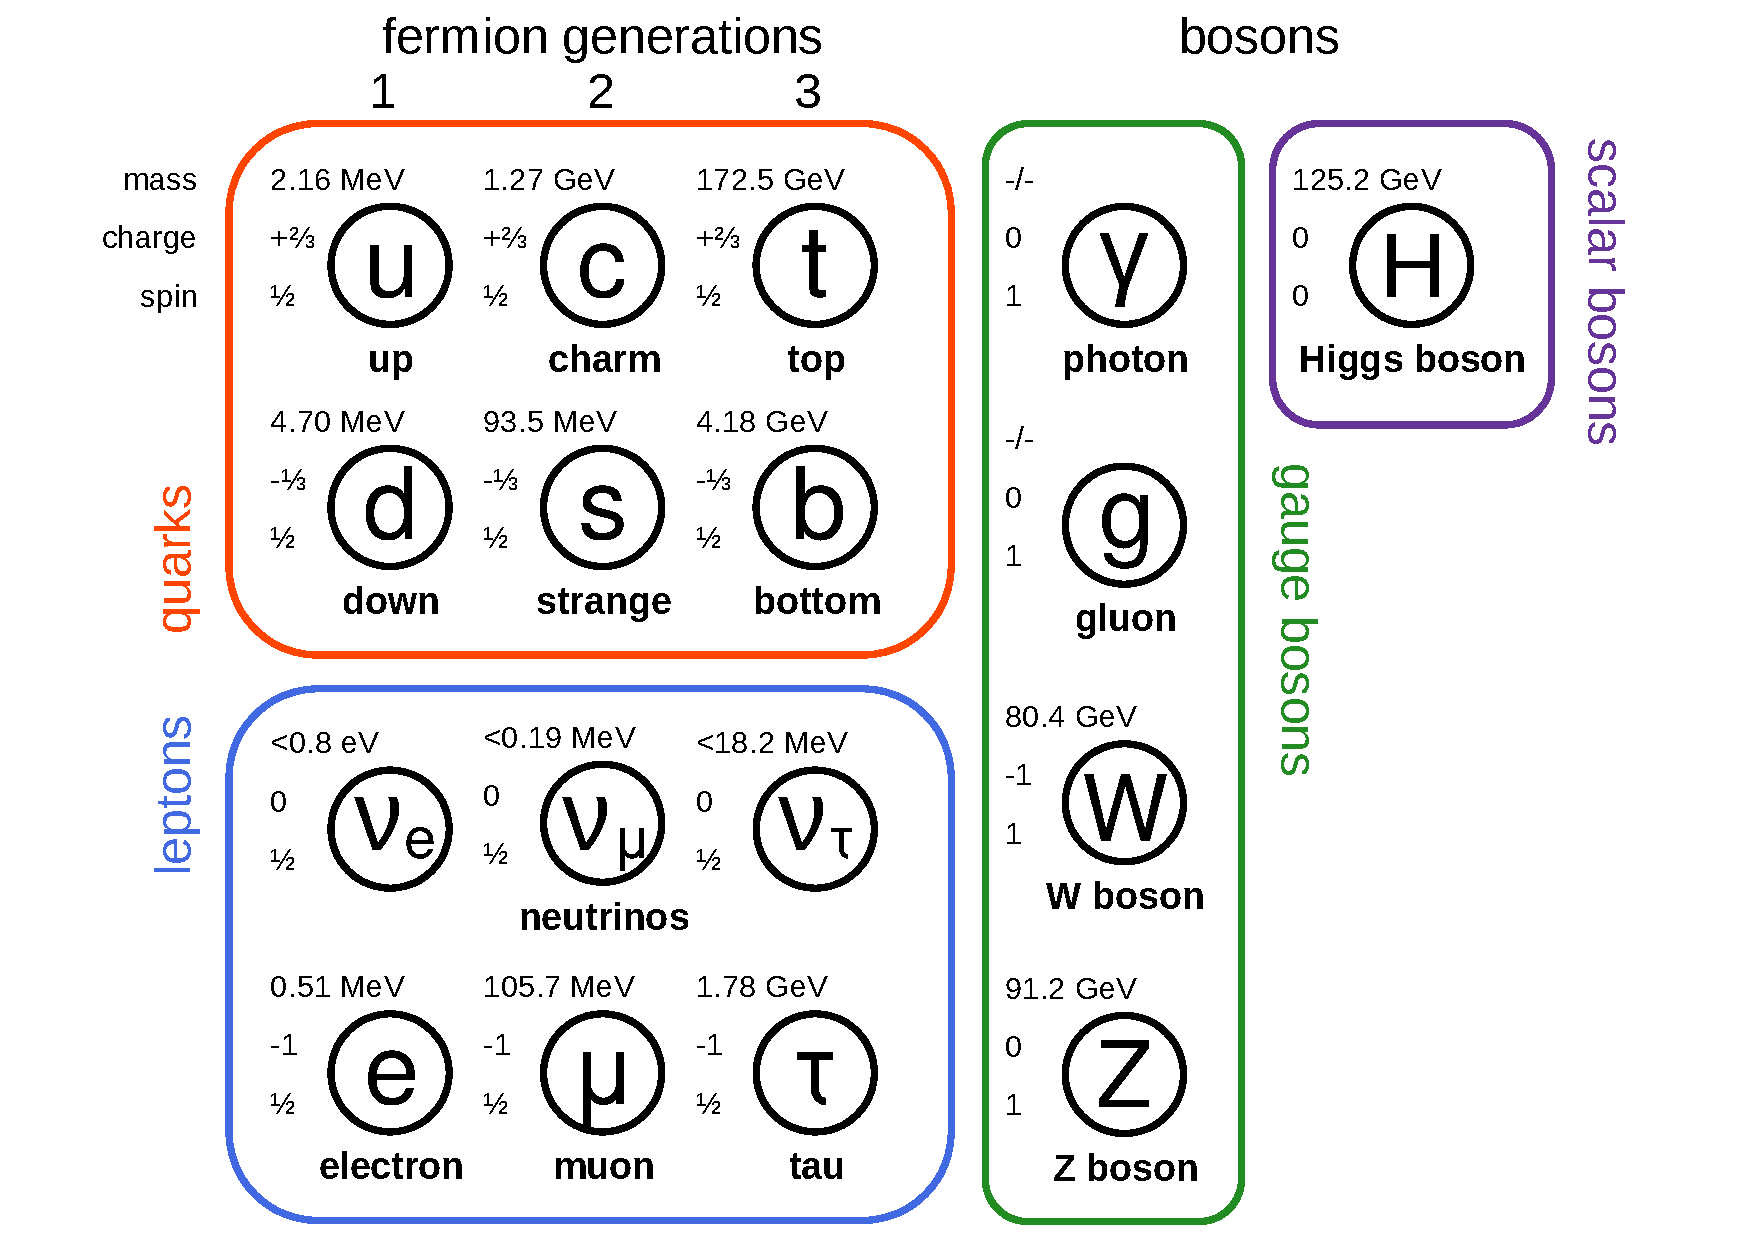
\includegraphics[width=0.9 \textwidth]{figures/smsketch_colors.pdf}
    \caption{\textbf{The Standard Model.} A schematic depiction of the particle content of the SM, showing the seventeen fundamental particles, split into six quarks, six leptons, four gauge bosons, and the Higgs boson. The mass, electromagnetic charge, and spin of the particles is given next to the labels. Mass information is taken from \citere{PDG:2022pth}.}
    \label{fig:theory:sm}
\end{figure}

The SM is formulated as a relativistic quantum field theory (QFT). That is, its most fundamental objects are fields acting on four-dimensional spacetime which, after a quantization procedure, yield physically observable particles as fundamental excitations. By the usual counting scheme, there exist seventeen different such fields, which can be classified into different groups, as schematically shown in \cref{fig:theory:sm}.

The first group consists of the twelve fermions, which have spin $\frac{1}{2}$ and make up all visible matter. They are further split into the leptons, consisting of three electrically charged leptons - electron, muon, and tau lepton - and three corresponding electrically neutral neutrinos, as well as the quarks, of which there are six different flavors, called up, down, strange, charm, bottom, and top. The quarks have fractional electric charge, and in addition carry color charge as their defining property. Of note is that the fermions are also split into three generations, with each generation consisting of a charged lepton, a neutrino, and two quarks. The only fundamental differences between the particles of different generations are their masses, though the resulting physically observable properties, such as the lifetime, might be dramatically different.

The second group of particles are the bosons, which have integer spin. Here, the four gauge bosons with spin 1 act as the force carriers of the four fundamental interactions described by the SM: the photon, for the electromagnetic interaction with coupling strength $\alpha_{\mathrm{elm}}$; the W and Z bosons, for the weak interaction with coupling strength $\alpha_W$; and the gluon, for the strong interaction with coupling strength $\alpha_S$. At high enough energies, the electromagnetic and weak interaction unify into the electroweak interaction (coupling strength $\alpha_{\mathrm{EW}}$). The last and final particle is the Higgs boson, which has spin 0. Its most important role in the SM is to give mass to the fermions, as well as the W and Z bosons, through the so-called Higgs mechanism~\cite{Higgs:1964ia,Englert:1964et}, which is briefly outlined in \cref{sec:theory:higgs}.

\subsection{Top quark}

This thesis focuses on one particular fundamental particle: the top quark. As such, it will be described in further detail in this section.

The top quark was first discovered in 1995 at the Tevatron by the CDF and D0 experiments~\cite{CDF:1995wbb,D0:1995jca}. With a rest mass of $m_t \approx \SI{172.5}{\GeV}$~\cite{ATLASCMS:2024dxp}, the top quark is the most massive known fundamental particle, and as a result it has unique properties compared to the other quarks: Its extremely short lifetime of $\sim \SI{5e-25}{\s}$ is lower than the typical time needed for a quark to hadronize under the strong interaction, making it the only bare quark - that is, the only quark which,  via its decay products, is observable outside of hadrons. Among others, a consequence of this is that it fully preserves spin information during its decay, while such information is typically lost for other quarks during hadronization. More details on this are found in \cref{sec:theory:spindensity}.

A second important property of the top quark that follows from its high mass is its large Yukawa coupling to the SM Higgs boson, which is of order one. As a result, the Higgs boson couples preferentially to the top quark of all SM fermions, and the study of both the SM Higgs boson and hypothetical additional Higgs bosons (see \cref{sec:theory:bsm}) is tightly connected to the top quark. 

In the SM, the top quark decays to a bottom quark and a W boson with a branching ratio (BR) of almost 100\% (to the degree that all other decays are commonly neglected). The W boson, in turn, can decay either to a charged lepton (e, $\mu$ or $\tau$) and the corresponding neutrino with a BR of $\sim32.6\%$, or to a pair of quarks (one up- and one down-type) with a BR of $\sim67.4\%$. This results in different final states for top production processes, which are discussed more in \cref{sec:theory:ttbar}.

\subsection{Higgs mechanism}
\label{sec:theory:higgs}

The Higgs boson is the most recently discovered particle of the SM. Its existence was confirmed in 2012 at the LHC by the ATLAS and CMS collaborations~\cite{ATLAS:2012tfa,CMS:HIG-12-028,CMS:HIG-12-036}, establishing the SM in its current form as the accepted description of elementary particle physics. In the SM, the Higgs boson is described by the so-called Higgs mechanism. It is briefly discussed in this section due to its relevance for many SM extensions involving additional Higgs bosons, as searched for in \cref{ch:ah,ch:alps}.

In the SM Lagrangian, the Higgs boson appears as a complex doublet $\phi$ in the form

\begin{equation}
    \mathcal{L}_{\mathrm{SM}} \subset \left(D_\mu \phi\right)^\dagger D^\mu \phi + V(\phi)
\end{equation}

\noindent where $D_\mu$ is the covariant derivative, containing the minimal coupling to the gauge fields, and the Higgs potential $V(\phi)$ is 

\begin{equation}
    V(\phi) = \mu^2 \phi^\dagger \phi - \lambda (\phi^\dagger \phi)^2 .
\end{equation}

Here, $\mu^2$ and $\lambda$ are free parameters of the model. If both parameters are positive, this potential (known as the ``Mexican hat potential'') has a minimum at a non-zero value of

\begin{equation}
    | \phi | = \frac{\mu}{\sqrt{2 \lambda}} \equiv \frac{v}{\sqrt{2}}
\end{equation}

\noindent with the vacuum expectation value $v = \mu / \sqrt{\lambda}$. On the other hand, the minimum - corresponding to the vacuum state - is degenerate with respect to the three phases (i.e. the $SU(2)$ symmetry) of the complex doublet.

In the Higgs mechanism, this symmetry is now spontaneously broken in the transition from the high-energy state of the early universe (where the minimum is at $|\phi| = 0$) to the low-energy state observed today. The physical particles after symmetry breaking are then described by fluctuations around the new vacuum state. If the Higgs field were to be considered on its own, this would lead to one massive (corresponding to fluctuations in the $|\phi|$ direction) and three massless degrees of freedom (corresponding to the phases).

However, the interaction with the electroweak gauge fields encoded within $D_\mu$ leads to the massless degrees of freedom being absorbed into the gauge fields. This turns three of the four massless spin-1 gauge fields of the electroweak Lagrangian (with two degrees of freedom each) into massive fields instead (which have an additional longitudinal polarization, and thus three degrees of freedom). These three massive gauge fields are identified with the W and Z bosons, while the remaining massless field is identified with the photon. Finally, the leftover massive degree of freedom from the Higgs doublet $\phi$ is identified with the spin-0 boson observed at the LHC.

The resulting masses of the Z, W and Higgs bosons can be calculated as a function of $\mu^2$, $\lambda$ and the electroweak couplings and thus used to test the Higgs mechanism. In addition to the electroweak bosons, the Higgs mechanism can also give masses to fermions (charged leptons and quarks) by including a Yukawa interaction term in the Lagrangian. This results in couplings between the SM Higgs boson and the different fermions that are proportional to the respective fermion mass. 

In many possible extensions of the SM, the simple Higgs mechanism as presented here is extended or replaced by more complex theories. This can lead to modifications to the Yukawa couplings, making Yukawa coupling measurements attractive as tests of the SM. Two examples of such extensions are discussed in \cref{sec:theory:twohdm,sec:theory:alps}.

\section{The \texorpdfstring{\pptt}{pp -> tt} process}
\label{sec:theory:ttbar}

In proton-proton collisions at the LHC, the dominant production mode of top quarks is the production of a top-antitop quark pair (\ttbar). The different parts of this thesis all focus on this process in different ways, and so this chapter gives a detailed overview of relevant effects.

At LO in QCD, there are three diagrams (up to permutations of initial and final states) contributing to \ttbar production, which can be seen in \cref{fig:theory:ttbar}. They differ in their initial states: the first two diagrams are induced by gluon fusion, while the last one is induced by quark fusion (mostly from $\mathrm{u \bar{u}}$ and $\mathrm{d \bar{d}}$). The fraction of these is determined by the corresponding parton densities; at a center-of-mass energy of $\sqrt{s} \geq \SI{13}{\TeV}$, gluon fusion dominates with a fraction of roughly 90\%.

\begin{figure}[t]
    \centering
    \begin{tikzpicture}[baseline=(current bounding box.center)]
      \begin{feynman}
        \vertex (i1) {\(g\)};
        \vertex [below=2.0 cm of i1] (i2) {\(g\)};
        \vertex [right=1.5 cm of i1] (a);
        \vertex [right=1.5 cm of i2] (b);
        \vertex [right=1.5 cm of a] (f1) {\(t\)};
        \vertex [right=1.5 cm of b] (f2) {\(\bar{t}\)};
        \diagram* {
          (i1) -- [gluon] (a),
          (i2) -- [gluon] (b),
          (f1) -- [anti fermion] (a) -- [anti fermion, edge label'=\(t\)] (b) -- [anti fermion] (f2)
        };
      \end{feynman}
    \end{tikzpicture}
    \hfill
    \begin{tikzpicture}[baseline=(current bounding box.center)]
      \begin{feynman}
        \vertex (a) ;
        \vertex [above left=1.3 cm of a] (i1) {\(g\)};
        \vertex [below left=1.3 cm of a] (i2) {\(g\)};
        \vertex [right=1.5 cm of a] (b);
        \vertex [above right=1.3 cm of b] (f1) {\(t\)};
        \vertex [below right=1.3 cm of b] (f2) {\(\bar{t}\)};
        \diagram* {
          (i1) -- [gluon] (a) -- [gluon] (i2),
          (a) -- [gluon, edge label'=\(g\)] (b),
          (f1) -- [anti fermion] (b) -- [anti fermion] (f2)
        };
      \end{feynman}
    \end{tikzpicture}
    \hfill
    \begin{tikzpicture}[baseline=(current bounding box.center)]
      \begin{feynman}
        \vertex (a) ;
        \vertex [above left=1.3 cm of a] (i1) {\(q\)};
        \vertex [below left=1.3 cm of a] (i2) {\(\bar{q}\)};
        \vertex [right=1.5 cm of a] (b);
        \vertex [above right=1.3 cm of b] (f1) {\(t\)};
        \vertex [below right=1.3 cm of b] (f2) {\(\bar{t}\)};
        \diagram* {
          (i1) -- [fermion] (a) -- [fermion] (i2),
          (a) -- [gluon, edge label'=\(g\)] (b),
          (f1) -- [anti fermion] (b) -- [anti fermion] (f2)
        };
      \end{feynman}
    \end{tikzpicture}
    \caption{\textbf{Feynman diagrams for \pptt.} The three diagrams (up to permutations) that contribute to the \pptt process at LO in QCD.}
    \label{fig:theory:ttbar}
\end{figure}

At NLO in QCD, many more diagrams become relevant, including those induced by the fusion of one quark and one gluon, while radiating a real quark. Similarly, real emissions of gluons can take place in $gg$ or $q\bar{q}$ fusion diagrams. These effects change the kinematic properties of the produced top quarks, leading to NLO corrections for predicted distributions.

After production, both the top and antitop quark in the \ttbar pair dominantly decay into a W boson and a b (anti)quark each. This leads to three different decay channels of the \ttbar pair depending on the decays of the two W bosons, which are classified according to their number of leptons: The dilepton channel, with final state $b \bar{b} \ell^+ \ell^- \nu \bar{\nu}$; the lepton+jets channel, with final state $b \bar{b} \ell \nu q \bar{q}$; and the all-hadronic channel, with final state $b \bar{b} q q \bar{q} \bar{q}$. Here, $q$ stands in for any light quark ($u$, $d$, $s$ or $c$).

The three channels differ greatly in their experimental challenges: The dilepton channel has the lowest branching ratio of $\sim10.6\%$, which is further reduced to $\sim6.4\%$ when excluding $\tau$ leptons decaying to hadrons due to then being experimentally hard to reconstruct. It also suffers from the fact that the two produced neutrinos escape the detector unobserved and are only measured as missing transverse momentum, losing both information in the forward direction as well as the ability to disentangle the two neutrinos. On the other hand, the final state of two opposite-sign charged leptons, two b jets, and missing transverse momentum does not have many other contributing processes in the SM, leading to very pure selections (particularly when the two leptons are an electron and a muon). All results in this thesis make use of this channel prominently.

By contrast, the lepton+jets channel has a large BR of $\sim43.9\%$ ($\sim30.4\%$ when excluding $\tau$ leptons decaying to hadrons), leading to high data statistics, and allows for easier interpretation of the missing transverse momentum due to only one neutrino. However, it can suffer from contamination by W+jets and multijet QCD background (the latter with non-prompt or fake leptons), from issues with combinatorics (i.e. the assignment of experimentally measured jets to the decay products) and from hadronic jet uncertainties, which can be large. This decay channel is employed for the result in \cref{ch:ttxs} as well as in the combination in \cref{ch:ah}.

Finally, the all-hadronic channel, with a similar BR of $\sim45.4\%$, is typically difficult to isolate from the background of QCD multijet production, and in addition suffers even more strongly from combinatorics and jet uncertainties then the lepton+jets channel. As a result, it is in many cases the least precise of the three channels, and is not studied further in this work.

\subsection{Spin state of the \ttbartitle system}
\label{sec:theory:ttbarspin}

As fermions with spin $\frac{1}{2}$, top quarks have two possible spin states. As a result, the relative spins of the \ttbar system can be either aligned, leading to a total vector state with spin $S = 1$, or anti-aligned, leading to a scalar state with spin $S = 0$. Furthermore, the \ttbar system as a whole can have orbital angular momentum $L$, where $L$ is a non-negative integer. In analogy to atomic orbitals, the total angular momentum is then $\vec{J} = \vec{L}+\vec{S}$, and for any chosen basis the set of quantum numbers $\{S,L,J,J_z\}$ consists of conserved quantities. The angular momentum state is commonly written using a term symbol ${}^{2S+1}L_{J}$, where $2S+1$ denotes the multiplicity of the spin state, and the orbital angular momentum $L$ is written using spectroscopic notation (S for $L=0$, P for $L=1$, D for $L=2$ etc). An overview of the lowest possible states ($J \leq 1$) is given in \cref{tab:theory:spinstates}, including also the parities and charge-parities $\mathcal{P}$ and $\mathcal{C}$, which can be inferred from the intrinsic parities of top and antitop as well as the orbital angular momentum. In proton-proton collisions, a mixture of all these states is produced, with the ratio depending on the production mode ($gg$, $q\bar{q}$ or $gq$) as well as the energy.

\begin{table}[]
    \centering
    \begin{tabular}{c|c|c|c}
         Term symbol & Spin multiplicity & $\mathcal{P}$ & $\mathcal{C}$ \\
         \hline
         \hline
         \term{1}{S}{0} & singlet & $-1$ & $+1$ \\
         \term{3}{P}{0} & triplet & $+1$ & $+1$ \\
         \term{3}{S}{1} & triplet & $-1$ & $-1$ \\
         \term{1}{P}{1} & singlet & $+1$ & $-1$ \\
         \term{3}{P}{1} & triplet & $+1$ & $+1$ \\
         \term{3}{D}{1} & triplet & $-1$ & $-1$
    \end{tabular}
    \caption{\textbf{Spin states of \ttbar.} Overview of the possible angular momentum states of the \ttbar system with $J \leq 1$, including the spin multiplicity, the parity $\mathcal{P}$ and the charge-parity $\mathcal{C}$.}
    \label{tab:theory:spinstates}
\end{table}


\begin{figure}[t]
    \centering
    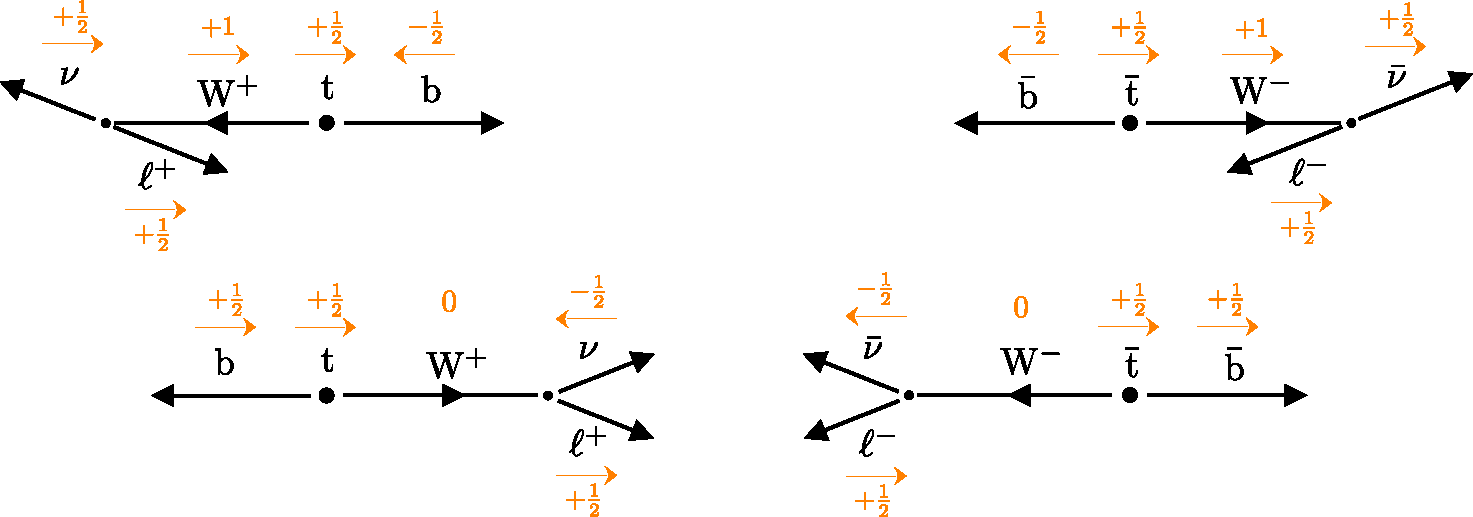
\includegraphics[width=0.95\linewidth]{figures/spin_corrs_sketch.pdf}
    \caption{\textbf{Helicity in top decays}. Sketch of the allowed helicity configurations in a top (left) and antitop quark decay (right) in the rest frame of the quark, involving either a transversely (top, $S_z = 1$) or longitudinally polarized W boson (bottom, $S_z = 0$). The $z$ axis corresponds to the spin of the top (anti)quark, and the orange arrows and numbers illustrate the spin in the $z$ direction of the respective particles. It can be seen that, due to conservation of angular momentum and the parity-violating nature of the weak interaction, the $\ell^+$ is preferred to be emitted in the direction of the $t$ spin, while the $\ell^-$ is preferred to be emitted opposite to the direction of the $\bar{t}$ spin.}
    \label{fig:theory:topspin}
\end{figure}

In practice, the spins of the top (anti)quarks cannot be observed directly, and instead must be inferred from their decay products. The way in which the spin information is passed to the decay products is determined by the maximally parity-violating nature of the weak interaction together with conservation of angular momentum. This is illustrated in \cref{fig:theory:topspin} for the leptonic decay of the top (anti)quark: Since the b quark is almost massless compared to the top quark, so that $m_{\mathrm{b}} = 0$ can be assumed in the following, it will be ultra-relativistic. Like for all fermions, its helicity is thus determined by its chirality. As a result, for the decay $t \rightarrow W^+ b$ the b quark - left-handed due to the weak interaction - has negative helicity (spin opposite to its direction of flight), leading to two possibilities for the W boson through conservation of angular momentum: transversely polarized (spin 1, top left in \cref{fig:theory:topspin}) or longitudinally polarized (spin 0, bottom left in \cref{fig:theory:topspin}).

Since the decay of the $W^+$ into $\ell^+ \nu$ is again mediated by the weak interaction, and both decay products are nearly massless, the helicities of $\ell^+$ and $\nu$ must be positive and negative, respectively. Applying again conservation of angular momentum, one then finds from the sketch that in both cases, the charged lepton is emitted preferably in the direction of the top quark spin. 

Repeating the same line of arguments for the decay of the antitop (\cref{fig:theory:topspin} on the right), one finds that the opposite holds there: the charged lepton is emitted preferably opposite to the antitop spin. As a result, the direction of flight of the charged lepton in the center-of-mass system of its parent (anti)top can be used as a proxy for the (anti)top spin (or, equivalently, its polarization). It should be noted that this property of the top quark is unique among the quarks of the SM, since all other quarks hadronize via the helicity-ignorant strong interaction and thus lose the largest part of their spin information\footnote{See e.g. \citere{Kats:2023zxb} for the greatly reduced possibilities of measuring spin correlations in \bbbar or \ccbar systems at the LHC.}.

Returning to the full \ttbar system, and applying the above observation to both top and antitop, one can now define observables to probe the \ttbar spin state, or equivalently, the spin correlation between $t$ and $\bar{t}$. A simple such variable is the azimuthal difference \dphill between the two leptons in a dileptonic decay. Assuming that the top and antitop are emitted back-to-back, a state with the top and antitop spins aligned (i.e. $S=1$) will cause the two leptons to be emitted preferably in opposite directions, leading to large \dphill, while anti-aligned spins ($S=0$) will lead preferably to parallel leptons and thus small \dphill. While this variable has the advantage of being easy to define and experimentally clean to measure, it is suboptimal in that it is also strongly affected by the kinematics of the \ttbar production, including higher-order corrections in QCD, and is heavily sculpted when selecting certain areas of \ttbar phase space. Thus, it is afflicted with large modeling uncertainties.

A more powerful variable can be defined by employing suitable reference systems as follows: the lepton and antilepton are first Lorentz boosted into the center-of-mass frame of the \ttbar system, and then further boosted into the center-of-mass frame of their parent (anti)tops. Then, a correlation variable \chel is defined as the scalar product of their direction unit vectors in these reference frames\footnote{
In this work, the naming convention from \citere{CMS:HIG-17-027} is followed for \chel. In e.g. \citere{Bernreuther:2004jv}, this variable is instead called $\cos \varphi$.
}:

\begin{equation}
\label{eq:theory:cheldef}
    \chel = \hat{\ell}^+_{t} \cdot \hat{\ell}^-_{\bar{t}} 
\end{equation}

It can be shown that, irrespective of the mode of production of the \ttbar system and inclusive in the rest of the phase space, the distribution of this observable always follows a straight line~\cite{Bernreuther:2004jv}, i.e.

\begin{equation}
\label{eq:theory:chel}
    \frac{1}{\sigma} \frac{d \sigma}{d \chel} = \frac{1}{2} \left( 1 - D \, \chel \right)
\end{equation}

The slope $D$ depends on the spin and angular momentum of the produced \ttbar state. At LO in QCD, it can be shown that $D=-1$ for pure singlet states (anti-aligned spins, e.g. \term{1}{S}{0}, \term{1}{P}{1}) and $D=+\frac{1}{3}$ for pure triplet states (aligned spins, e.g. \term{3}{S}{1}, \term{3}{P}{0})~\cite{Maltoni:2024tul,Cheng:2024btk}. Higher-order corrections in QCD can slightly reduce these slopes through emissions of real gluons in the decay, which weaken the correlations, but these effects are on the order of $0.2\%$ at NLO for leptons~\cite{Czarnecki:1990pe,Bernreuther:2003ga}. %For states with orbital angular momentum, there is an additional degree of freedom in the decay since only the total angular momentum with respect to any axis is conserved. As a result, the slopes $D$ for these states are less steep; for example, the \term{3}{P}{0} state (with aligned spins) has a mildly negative slope of \todo{}.

In practice, any observed ensemble of \ttbar pairs will be a mixture of the different spin states depending on the production mechanism and underlying theory, which can be probed by measuring the slope $D$. As will be discussed in \cref{sec:theory:bsm}, extensions of the SM can change the predicted slope, making measurements of $D$ attractive tests for new physics. The value of $D$ has been measured e.g. in \citeres{CMS:TOP-14-023,CMS:TOP-18-006,CMS:TOP-23-007}, as well as more recently as a proxy variable in the context of measurements of quantum entanglement in \ttbar production~\cite{CMS:TOP-23-001,ATLAS:2023fsd}.

%$\todo{measurements of D, entanglement}

\subsection{Spin density matrix}
\label{sec:theory:spindensity}

A more detailed way to quantify the spin properties of the \ttbar system, respective to an arbitrary spin basis, is the production spin density matrix $\mathbf{R}$, which (when averaged over initial spins and colors, and summed over final colors) can be written as~\cite{Maltoni:2024tul,Cheng:2024btk,Anuar:PhD}

\begin{equation}
    \mathbf{R} = A \, \mathbb{1} \otimes \mathbb{1}
    + B_i^1 \, \sigma_i \otimes \mathbb{1}
    + B_i^2 \, \mathbb{1} \otimes \sigma_i
    + C_{ij} \, \sigma_i \otimes \sigma_j.
\end{equation}

Here, $\mathbb{1}$ is the two-dimensional identity matrix, $\sigma_i$ with $i=1,2,3$ are the Pauli matrices, and the first and second components of the tensor product refer to the spin of the top and antitop quark, respectively. The scalar coefficient $A$ describes the overall amplitude (i.e. the differential cross section as a function of the top and antitop kinematics) of \ttbar production, the vectors $\vec{B}^1$ and $\vec{B}^2$ describe the polarization of the top and antitop quark, and the matrix $\mathbf{C}$ describes the correlation between their spins. All of them are, in general, functions of the partonic center-of-mass energy and the scattering angle of the top quark relative to the incoming partons.

As explained in \cref{sec:theory:ttbarspin}, in a dileptonic decay the spin information is transferred almost completely to the charged leptons. Defining the lepton directions of flight in their parent frames $\hat{\ell}_t^+$ and $\hat{\ell}_{\bar{t}}^-$ as in \cref{eq:theory:cheldef}, the resulting differential cross section in terms of the lepton angles, collectively denoted as $\Omega$, is~\cite{Anuar:PhD}

\begin{equation}
    \frac{1}{\sigma} \frac{d \sigma}{d \Omega} = 1 + \vec{B}^1 \cdot \hat{\ell}_t^+ + \vec{B}^2 \cdot \hat{\ell}_{\bar{t}}^- + (\hat{\ell}_t^+)^T \, \mathbf{C} \, \hat{\ell}_{\bar{t}}^- .
\end{equation}

By integrating out the remaining angles, it can be shown from this that irrespective of the chosen basis the slope $D$ as defined in \cref{eq:theory:chel} can be recovered from the matrix $\mathbf{C}$ as~\cite{Bernreuther:2004jv,Bernreuther:2017yhg}

\begin{equation}
    D = \frac{1}{3} \mathrm{Tr} \left[ \mathbf{C} \right] .
\end{equation}

\begin{figure}[t]
  \centering
  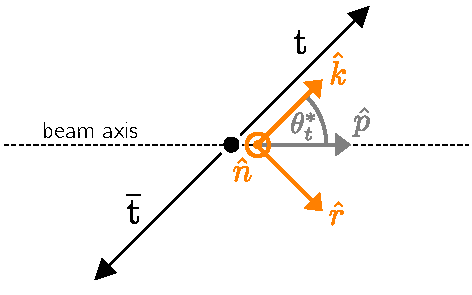
\includegraphics[width=0.6\linewidth]{figures/helicity_basis_new.pdf}
  \caption{\textbf{Helicity basis.} Sketch of the helicity basis used to define the top and antitop quark spins. The unit vectors $\hat{k}$, $\hat{r}$ and $\hat{n}$ define the right-handed basis, while the beam axis is given by $\hat{p}$ and the top quark scattering angle by $\theta^*_t$.}
  \label{fig:theory:helicitybasis}
\end{figure}

As discussed in \cref{sec:theory:ttbarspin}, $D$ is maximally negative for pure singlet states (corresponding to a positive slope in \chel), and thus is ideal for separating those in a mixed ensemble. One can define similar separating observables for other states using the spin density matrix by choosing a suitable spin basis. In this work, the so-called helicity basis proposed in \citere{Bernreuther:2015yna} is used. The three axes of this basis, denoted $\hat{k}$, $\hat{r}$ and $\hat{n}$, are defined as follows: $\hat{k}$ is simply the direction of flight of the top quark in the center-of-mass frame of the \ttbar system, such that the top quark spin with respect to $\hat{k}$ is equal to the helicity. The second axis, $\hat{r}$, is orthogonal to $\hat{k}$ in the scattering plane of the \pptt process. Finally, the third axis $\hat{n}$ is orthogonal on both $\hat{k}$ and $\hat{r}$, oriented such that the $\{\hat{k},\hat{r},\hat{n}\}$ system is left-handed. If $\hat{p}$ denotes the beam axis and $\theta^*_t$ the top scattering angle, the latter two axes are given by

\begin{equation}
    \hat{r} = \frac{\hat{p} - \cos \theta^*_t \hat{k}} {| \hat{p} - \cos \theta^*_t \hat{k} |} \quad \mathrm{and} \quad \hat{n} = \hat{r} \times \hat{k} = \frac{\hat{p} \times \hat{k}} {| \hat{p} \times \hat{k} |}.
\end{equation}

This coordinate system is visualized in \cref{fig:theory:helicitybasis}. It is used, among others, in \citeres{CMS:TOP-18-006,CMS:TOP-23-007} to measure both the polarizations $\vec{B}^1$ and $\vec{B}^2$ and spin correlation coefficients $C_{ij}$ ($i,j = k,r,n$). In this work, only the spin correlation is considered. Particularly, in addition to \chel, the following observable is defined:

\begin{equation}
    \label{eq:theory:chan}
    \chan = - (\hat{\ell}_t^+)_k (\hat{\ell}_{\bar{t}}^-)_k + (\hat{\ell}_t^+)_r (\hat{\ell}_{\bar{t}}^-)_r + (\hat{\ell}_t^+)_n (\hat{\ell}_{\bar{t}}^-)_n
\end{equation}

\noindent where $(\hat{\ell})_i$, $i=k,r,n$ refers to the $i$-th component of the respective vector in the $\{k,r,n\}$ basis. This observable, like \chel, has the advantage of always being linear in the absence of phase space cuts, i.e.

\begin{equation}
    \frac{1}{\sigma} \frac{d \sigma}{d \chan} = \frac{1}{2}\left( 1 + D^{(k)} \chan \right)
\end{equation}

\noindent where~\cite{Maltoni:2024tul}

\begin{equation}
\label{eq:theory:Dk}
    D^{(k)} = \frac{1}{3} \left( C_{kk} - C_{rr} - C_{nn} \right) .
\end{equation}

From \cref{eq:theory:Dk}, it can be seen that the slope is maximally negative, $D^{(k)} = -1$, when the top and antitop spins are anti-correlated along the top direction of flight ($C_{kk} = -1$) and correlated along the orthogonal directions ($C_{rr} = C_{nn} = +1$). The (unpolarized) state described by these correlations is a pure triplet state ($S=1$)~\cite{Maltoni:2024tul}. 

Particularly, the \term{3}{P}{0} state of \ttbar always corresponds to this spin state: It has no total angular momentum, so that its total spin and orbital angular momentum must be anti-aligned. Since the orbital angular momentum is always exactly zero in the direction of flight of the top quarks, the \ttbar system must be in an orbital angular momentum eigenstate with $L_k = 0$, and thus also in a total spin eigenstate with $S_k = 0$. In other words, the spins in the $\hat{k}$ direction are anti-aligned, corresponding to $C_{kk} = -1$. In order to arrive at $S=1$, i.e. a pure triplet state, it is required that the other entries fulfill $C_{rr} = C_{nn} = 1$.


% next: a) choice of basis - helicity basis by Bernreuther
% b) decay products - weak interaction (V-A), ??? try to understand this shit

\subsection{Bound state effects in \ttbartitle}
\label{sec:theory:etat}

When predicting distributions of observables for hard scattering processes such as \ttbar production, one usually employs perturbative calculations at a fixed order in the strong coupling constant \alphas, possibly matched to a parton shower (see \cref{ch:mc}). However, at low energy scales (or equivalently, long distances) the strong interaction becomes non-perturbative, leading to effects that cannot be captured in the usual perturbative expansion irrespective of the order in \alphas (though they might or might not be captured in expansions or resummations with other parameter choices).

In the \pptt process, such effects might play a role in the vicinity of the \ttbar production threshold, i.e. for $\mtt \sim 2 \mt$, where the relative velocities of the produced top quarks become small. In particular, one possible class of effects not included in simple expansions in \alphas are \ttbar bound states (``toponium''). Such states (also called quarkonia) are well-known in \ccbar and \bbbar production, where they lead to composite particles such as $\mathrm{J/\psi}$, $\eta_c$ or $\Upsilon$. When translating this knowledge to \ttbar, however, there is a significant difference: due to the large top quark mass, the lifetime of the top quark is expected to be shorter than the (formal) lifetime of any possible \ttbar bound state. As a result, the state would in the majority of cases not decay e.g. to photons, gluons or hadrons like the lighter quarkonia, but instead disassociate by one of the constituent top quarks decaying normally to Wb. This phenomenon, sometimes called a ``quasi-bound state'' or a ``virtual bound state", would lead to a possible peak in the \mWWbb spectrum slightly below the \ttbar threshold.

Calculations of the \mWWbb spectrum at the \ttbar threshold including the effects from a possible bound state have been performed independently in \citeres{Fadin:1990wx,Kiyo:2008bv,Sumino:2010bv,Ju:2020otc,Garzelli:2024uhe}. All of these calculations work in the framework of non-relativistic QCD (NRQCD), which treats the slowly moving ($v \ll c$) top (anti)quarks as non-relativistic particles. This approach can be seen as a low-energy effective field theory (EFT) of the SM where high-energy modes have been integrated out, or alternatively, as an alternate perturbative expansion in the ratio $\alphas/\beta$, where $\beta$ is the top quark velocity. The result is a non-relativistic Schr\"odinger equation for the wavefunction of the \ttbar system, with the interaction between the top quarks described by the low-energy limit of the QCD Coulomb potential, representing the exchange of soft gluons. At LO, it is given by~\cite{Kiyo:2008bv}

\begin{equation}
    V_{\mathrm{QCD}}^{[1,8]} (q) = - \frac{4 \pi \alphas C^{[1,8]}}{q^2} ,
\end{equation}

\noindent where the color factor is $C^{[1]} = 4/3$ for color-singlet and $C^{[8]} = -1/6$ for color-octet states. As a result, only \ttbar systems in a color-singlet state feel an attractive force and can possibly form a bound state, while color-octet states are instead repulsed. At the LHC, \ttbar bound states can thus at LO be produced only from gg initial states, since \qqbar systems are always color-octets. From this, the spin state of the produced bound state can be inferred: Since both of the top quarks have low velocity, states with orbital angular momentum $L \neq 0$ will be strongly suppressed (beyond NLO in NRQCD~\cite{Kiyo:2008bv}). Furthermore, the gg initial state in \ttbar production close to the \ttbar threshold always has spin $S = 0$ (and thus total angular momentum $J = 0$), with $S = 2$ contributions suppressed by powers of the top velocity~\cite{Cheng:2024btk}, so that the resulting \ttbar system must be in the \termc{1}{S}{0}{1} state. At NLO in QCD, also \termc{3}{S}{1}{1} states can be produced; however, the contribution is very small (less than $0.1\%$ of the total cross section~\cite{Kiyo:2008bv}).

\citeres{Kiyo:2008bv,Sumino:2010bv,Ju:2020otc,Garzelli:2024uhe} agree that the binding energy of the \ttbar bound state, defined as the difference of the peak position in the \mWWbb spectrum to $2 \mt$, is around \SI{-2}{\GeV}, resulting in a ``mass'' of \SI{343}{\GeV} for the \ttbar bound state for a top mass of \SI{172.5}{\GeV}. The exact line shape of the peak is less well known. However, the experimental resolution of \mWWbb is expected to be much larger than the bound state width of order $\sim 2 \Gamma_t$ (see \cref{sec:ah:kinreco}), making the details of the spectrum irrelevant to an experimental search.

The existing NRQCD calculations predict only certain differential distributions and cannot be directly compared to experimental data on a per-event level. Because of this, a simplified model for the \ttbar bound state is introduced following \citeres{Maltoni:2024tul,Maltoni:2024csn,Fuks:2021xje,Aguilar-Saavedra:2024mnm}. Instead of a first-principles calculation, the bound state effects are modeled as an additional state spin-0 state \etat, which is added to the conventional perturbative QCD (pQCD) calculation of \ttbar. \etat is defined to couple directly to gluons and top quarks via the Lagrangian

\begin{equation}
\label{eq:theory:etatlagrangian}
  \mathcal{L}_{\etat} = - \frac{1}{4} g_{\mathrm{gg} \etat} \etat G^{a}_{\mu \nu} \tilde{G}^{a \mu \nu} - i g_{\ttbar \etat} \etat \bar{t} \gamma_5 t
\end{equation}

\noindent where $G^{a}_{\mu \nu}$ is the gluon field strength tensor, $\tilde{G}^{a}_{\mu \nu}$ its dual, and $g_{\mathrm{gg} \etat}$ as well as $g_{\ttbar \etat}$ are arbitrary coupling strengths. The resulting model has three free parameters: the binding energy $E_b = \metat - 2 \mt$, the total width \Gammaetat and the production cross section $\sigma(\etat)$ (the latter determining the couplings $g_{\mathrm{gg} \etat}$ and $g_{\ttbar \etat}$). In \citere{Fuks:2021xje}, they are determined by fitting them to the NRQCD calculation from \citere{Sumino:2010bv}, yielding

\begin{equation}
  \label{eq:theory:etatparams_7gev}
  E_b = \SI{-2}{\GeV} \implies \metat = \SI{343}{\GeV}, \quad \Gammaetat = \SI{7}{\GeV}, \quad \sigma(\etat) = \SI{6.4}{\pb}
\end{equation}

In the generation of events, the top quarks are allowed to be fully off-shell by calculating the full amplitude $p p \rightarrow \etat \rightarrow W^+ W^- b \bar{b}$, thus making sure that the phase-space region $\mWWbb < 2 \mt$ is populated. Furthermore, \citere{Fuks:2021xje} recommends that the contribution of \etat should be restricted to the region $|\mWWbb - \metat| \leq \SI{6}{GeV}$ so that the bulk of the \ttbar phase space, in which the pQCD calculation is expected to be accurate while the NRQCD calculation misses relativistic corrections, is not affected.

However, \citeres{Maltoni:2024csn,Aguilar-Saavedra:2024mnm} recommend instead

\begin{equation}
  \label{eq:theory:etatparams_2p8gev}
  E_b = \SI{-2}{\GeV} \implies \metat = \SI{343}{\GeV}, \quad \Gammaetat = 2 \Gamma_{t} = \SI{2.8}{\GeV}
\end{equation}

\noindent and no cut on $|\mWWbb - \metat|$.

\begin{figure}[t]
    \centering
    %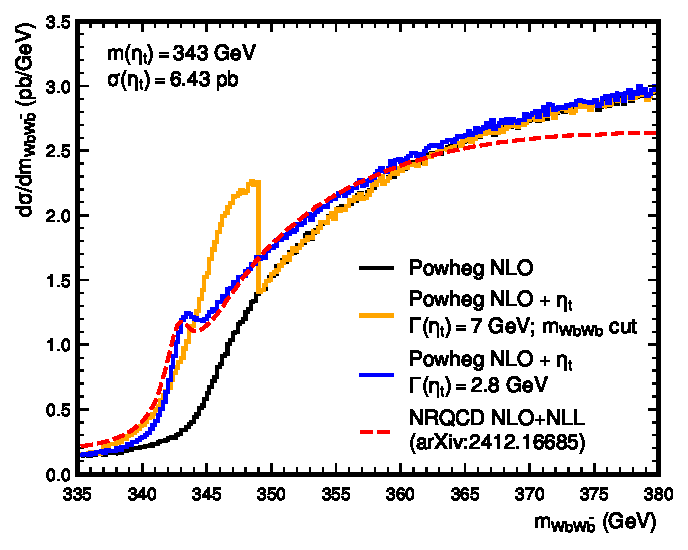
\includegraphics[width=0.8\linewidth]{figures/ah/powheg_etat_nlo.pdf}
    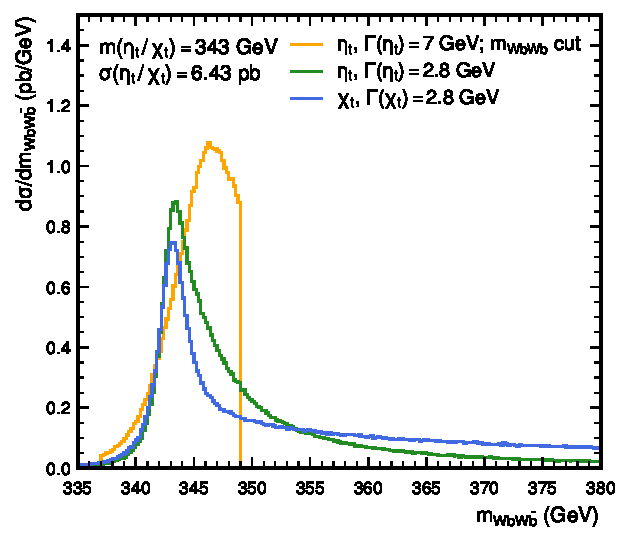
\includegraphics[width=0.49\linewidth]{figures/ah/etat_chit_small.pdf}
    \hfill
    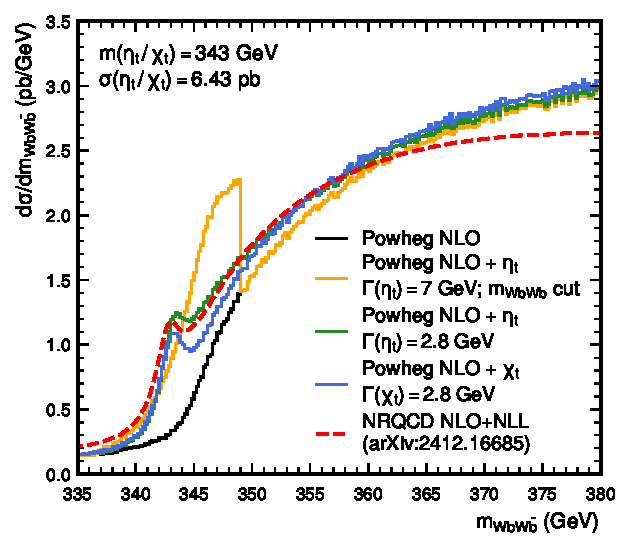
\includegraphics[width=0.49\linewidth]{figures/ah/powheg_etat_nlo_small.pdf}
    \caption{\textbf{Line shape of \etat and \chit.} The \mWWbb distribution close to the \ttbar threshold, as predicted by the \etat and \chit models on their own (left) and stacked on top of a pQCD \ttbar prediction from Powheg \hvq (right, see \cref{sec:mc:me}). For the orange line, the \etat width is chosen to be \SI{7}{\GeV}, and a cut on $|\mWWbb - \metat|$ is applied (\cref{eq:theory:etatparams_7gev}), while for the green line, the \etat width is chosen as \SI{2.8}{\GeV}, and no further cuts are made (\cref{eq:theory:etatparams_2p8gev}). The blue line shows \chit for a width of \SI{2.8}{\GeV}. In the right plot, all models are compared to an NRQCD prediction from \citere{Garzelli:2024uhe}.}
    \label{fig:theory:etat}
\end{figure}

The resulting \mWWbb distribution for the combination of pQCD \ttbar and \etat is shown in \cref{fig:theory:etat} at the level of hard scattering for both parameterizations, on its own as well as stacked on top of a pQCD prediction of the \ttbar continuum at NLO in QCD. The stacked distributions are compared to an NRQCD prediction from \citere{Garzelli:2024uhe}.
%In addition to the parameters given in \cref{eq:theory:etatparams}, a case with a lower width of $\Gamma_{\etat} = \SI{2.8}{\GeV}$ is also shown. 
At the level of hard scattering, the lower width of $\Gammaetat = 2 \Gamma_t$ agrees much better with the predicted NRQCD spectrum and avoids an unphysical discontinuity due to the \mWWbb cutoff. Thus, this parameterization will be used in this work wherever possible, i.e. in \cref{sec:ah:excess,sec:ah:limits}, though the parameterization of \cref{eq:theory:etatparams_7gev} is retained for the sake of consistency with other results in \cref{sec:ah:combination}. For more details, see these sections.

In the final stages of this work, a more involved model for \ttbar bound states was published in \citere{Fuks:2024yjj}. There, instead of simulating an additional pseudoscalar state \etat, the bound state effects are included in leading-order color-singlet \ttbar production by directly reweighting produced events with the ratio of Green's functions. This model is in principle fully predictive, i.e. it does not require fitting parameters to external calculations. However, it could not be validated in time for inclusion in the results of \cref{ch:ah}, it does not explicitly distinguish between \ttbar spin states, and it is also unclear on how to match it to the \ttbar continuum. Because of this, it is not further considered here and its investigation left for future work.
%\todo{decide on how to treat 7 and 2.8 GeV in the end}
%However, already after parton showering the difference between the cases is negligibly small due to smearing from intial and final state radiation. At detector level, this smearing is expected to increase even more due to the rather coarse experimental resolution of the \mtt reconstruction (see \cref{sec:ah:kinreco}). In general, the experimental signature of \etat will be mostly independent on the assumed mass and width in the considered ranges. Because of this, the original specification from \citere{Fuks:2021xje} is deemed sufficient and used in the remainder of this work.

While NRQCD predicts any possible \ttbar bound state contribution in pp collisions to be dominated by the \termc{1}{S}{0}{1} state, with contributions from excited states strongly suppressed, experimentally it will still be useful to compare this spin state to other possibilities. To this end, a second toy model, denoted \chit, is defined in analogy to \etat by the interaction Lagrangian

\begin{equation}
  \mathcal{L}_{\chit} = - \frac{1}{4} g_{\mathrm{gg} \chit} \chit G^{a}_{\mu \nu} \tilde{G}^{a \mu \nu} - g_{\ttbar \chit} \chit \bar{t} t
\end{equation}

\noindent where $g_{\mathrm{gg} \chit}$ and $g_{\ttbar \chit}$ are again arbitrary couplings. This Lagrangian contains a \CP-even coupling to the top quark, compared to the \CP-odd coupling in \cref{eq:theory:etatlagrangian}. It thus produces \ttbar systems in the \termc{3}{P}{0}{1} state, which is the only other possible state with $J = 0$ (cf. \cref{tab:theory:spinstates}). The free parameters of this model are again cross section, mass, and width; they are set here to the same values as for \etat in all cases\footnote{Based on analogies to \ccbar and \bbbar quarkonia~\cite{Barnes:2005pb}, it is likely that a true \term{3}{P}{0} bound state would have a slightly higher mass, though it is unknown whether this would be noticeable even in the hard-scattering level spectrum due to the large smearing from the top width. It is anyway expected to be irrelevant within the experimental resolution.}. The resulting \mWWbb line shape is also seen in \cref{fig:theory:etat}. It shows a small peak similar to \etat at $\sim \SI{343}{\GeV}$, though it exhibits a more pronounced tail at high \mWWbb since the \term{3}{P}{0} state carries one unit of orbital angular momentum and thus favors higher top quark velocities. In \cref{sec:ah:parityscan}, the \chit model will be used in conjunction with \etat to probe the spin state of the observed excess. Other possible states, such as the vector state \termc{3}{S}{1}{1}, are not considered here and instead left for future work.

% perturbative vs non-perturbative
% quarkonia: J/Psi, Upsilon
% also for ttbar? lifetime very short - might decay before bound state forms

% formalism: pNRQCD
% what actually is that? Greens fct ? resummation in alphas/beta ?
% problem: top is unstable - width ~ binding energy, cannot neglect

% consider pseudoscalar (i.e. spin-singlet) state - largest at LHC
% color-singlet vs color-octet: only the singlet potential is attractive
% --> color-octet contributions dont give resonances
% can get gq -> singlet or even qq -> singlet in NLO, but small

% Predicted: binding energy ~ 2 GeV

% difficulties: how to match to relativistic regime?
% how to treat soft gluon emissions ?
% how to treat off-shell tops / interference with tW / WWbb ?

% mass resolution at LHC is poor - dont need details of the spectrum
% --> model as generic pseudoscalar state eta_t coupling directly to gg and ttbar - this is just a toy model
% note that seperation ``ttbar'' vs ``etat'' is nonphysical
% i.e. parametrize the enhancement through bound-state effects by etat


\section{Beyond the Standard Model}
\label{sec:theory:bsm}

The Standard Model, greatly successful as it is at describing the results of collider experiments so far, is nonetheless known to be incomplete. In fact, there exist several experimental results which cannot be explained by SM predictions, such as the observation of dark matter in many astrophysical contexts~\cite{Bertone:2004pz,Porter:2011nv,Arbey:2021gdg} or the observed masses of the neutrinos~\cite{deGouvea:2016qpx,Dev:2023iyn}. 

In addition, the SM is plagued by several theoretical challenges that will likely not be overcome without major modifications to the theory. Chief among these is the unification of the forces of the SM - the electroweak and strong interactions - with gravity as described by General Relativity, which is not included in the SM at all. Doing so has proven extremely challenging, and no fully consistent unified theory of all forces is known yet. Further open questions are, for example, the hierarchy or naturalness problem~\cite{Nelson:1985,Koren:2020pio,Craig:2022eqo} or the strong \CP problem~\cite{Peccei:1977hh,Peccei:1977ur}.

In order to solve these problems in a satisfactory manner, a more general theory will have to be found, which should include the SM as its low-energy limit. In many cases, this will result in additional as of yet undiscovered particles. There is a multitude of such Beyond the Standard Model (BSM) extensions, each attacking different parts of the problems, and one of the major tasks of particle physics is to explore which parts of the parameter space of these models can be probed with the current experiments.

This work, in particular, aims to probe models predicting new, heavy spin-0 states coupling strongly to the top quark. Such states can be searched for in the \pptt process, as outlined in a generic fashion in \cref{sec:theory:ah}. Following that, two explicit realizations of such models are discussed, namely the Two-Higgs Doublet Model (2HDM) (\cref{sec:theory:twohdm}) and Axion-Like Particle (ALP) models (\cref{sec:theory:alps}).

\subsection{Heavy scalars in \ttbartitle production}
\label{sec:theory:ah}

Consider an unspecified BSM extension predicting (possibly among others) a massive spin-0 state $\Phi$ coupling to top quarks via a Yukawa interaction. In the absence of couplings to other particles, the Lagrangian of such a state can be written as~\cite{Maltoni:2024tul}

\begin{equation}
\label{eq:theory:lag_ah}
    \mathcal{L}_{\Phi} = \, \frac{1}{2} (\partial_\mu \Phi ) (\partial^\mu \Phi ) +\frac{m_{\Phi}^2}{2} \Phi^2 
    + g_{\mathrm{\Phi \bar{t} t}} \frac{\mt}{v} \bar{t} \Phi \left( \cos{\alpha} + i \gamma_5 \sin{\alpha} \right) t .
    %+ i  \gAtt \, \frac{\mt}{v} \bar t  \gamma_5 \, t  \, \Phi 
    %-  \gHtt \, \frac{\mt}{v} \bar t \, t  \, \Phi .
\end{equation}

\noindent where $m_\Phi$ is the mass of the new state and $g_{\mathrm{\Phi \bar{t} t}}$ is a coupling modifier, scaled to the SM Higgs-top Yukawa coupling with the SM Higgs vacuum expectation value $v$. The phase $\alpha$ is a free parameter determining the \CP structure of the $\Phi \bar{t} t$ coupling: For $\alpha = 0$, the coupling is purely \CP-even or scalar, while for $\alpha = \pi/2$, the coupling is purely \CP-odd or pseudoscalar. Intermediate values for $\alpha$ will cause \CP-mixed couplings, which in general will result in  \CP violation in processes involving top quarks. Possible experimental indicators of such \CP violation in \pptt are e.g. discussed in \citere{Bernreuther:2017yhg}.

\begin{figure}[!t]
    \centering
    \begin{tikzpicture}[baseline=(current bounding box.center)]
      \begin{feynman}
        \vertex (i1) {\(g\)};
        \vertex [below=2.0 cm of i1] (i2) {\(g\)};
        \vertex [right=1.5 cm of i1] (a);
        \vertex [right=1.5 cm of i2] (b);
        \vertex [below right=1.0 cm and 1.73 cm of a] (c);
        \vertex [right=2.0 cm of c] (d);
        \vertex [right=5.46 cm of a] (f1) {\(t\)};
        \vertex [right=5.46 cm of b] (f2) {\(\bar{t}\)};
        \diagram* {
          (i1) -- [gluon] (a),
          (i2) -- [gluon] (b),
          (c) -- [anti fermion] (a) -- [anti fermion, edge label'=\(t\)] (b) -- [anti fermion] (c),
          (c) -- [scalar, edge label'=\(A/H\)] (d),
          (f1) -- [anti fermion] (d) -- [anti fermion] (f2)
        };
      \end{feynman}
    \end{tikzpicture}
    \caption{\textbf{Feynman diagram for $\mathrm{gg \rightarrow A/H \rightarrow \ttbar}$.} Only the leading-order gluon fusion diagram is shown, with a top quark running in the loop.}
    \label{fig:theory:ggAH}
\end{figure}

In the scope of this work, only the \CP-conserving cases of $\Phi$ are considered. For convenience, the pure pseudoscalar case will in the following be called A, while the pure scalar case will be called H.

Similar to the SM Higgs boson, the most important production channel of either state at the LHC will be through loop-induced gluon fusion, followed by associated production with either \ttbar or a single top quark. Only the former is considered here; experimental searches for the latter case can be found e.g. in \citere{CMS:EXO-22-014-PAS}. Furthermore, the decay of the new state will depend on its mass: For low masses, the particle will decay either through loop-induced couplings to e.g. gg or $\gamma \gamma$ or, if present, through couplings to other SM or BSM particles than the top quark. For masses of $\mAH > 2 \mt$, however, the decay to \ttbar is kinematically allowed and will in many cases be dominant due to the large Yukawa coupling. In this case, the process $\mathrm{gg \rightarrow A/H \rightarrow \ttbar}$ will lead to the same final state as SM \ttbar production, as illustrated in \cref{fig:theory:ggAH}. This process will be considered in more detail in the rest of this chapter, and one of the main results of this thesis is an experimental search for such a signature (\cref{ch:ah}).



\begin{figure}[ht!]
    \centering
    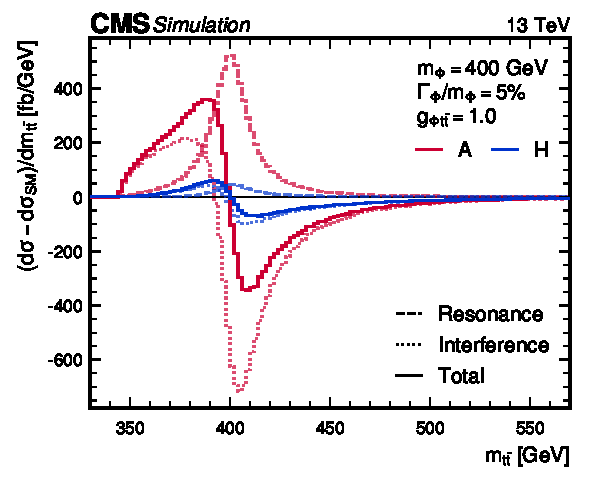
\includegraphics[width=0.49\linewidth]{figures/ah/ah_xs/ahspectrum_400.pdf}
    \hfill
    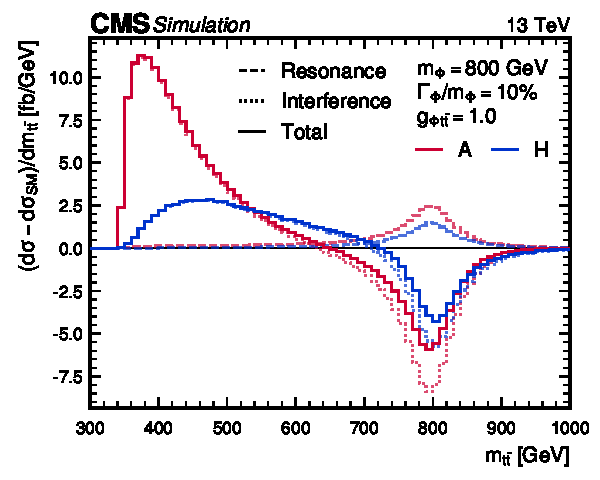
\includegraphics[width=0.49\linewidth]{figures/ah/ah_xs/ahspectrum_800.pdf}
    \caption{\textbf{Differential cross sections for $\mathrm{A/H} \rightarrow \ttbar$.} The hadronic differential cross section as a function of the invariant \ttbar mass, with the SM prediction subtracted, for $\mAH = \SI{400}{GeV}$, $\wAH/\mAH = 5\%$(left) and $\mAH= \SI{800}{\GeV}$, $\wAH/\mAH = 10\%$ (right) as well as for A (red) and H (blue), at a coupling modifier of $\gAHtt = 1$. The resonance and interference components as well as their sum are shown as dashed, dotted and solid lines, respectively. They are calculated from same the Monte Carlo simulation samples described in \cref{sec:ah:datasets}.}
    \label{fig:theory:ahxs}
\end{figure}

\cref{fig:theory:ahxs} shows the predicted differential cross sections of this model in terms of \mtt, the invariant mass of the \ttbar pair, for different A/H masses. The cross section is shown as the difference to the SM prediction at the level of the hard scattering and at LO in QCD. It can be seen that the total effect of A and H is a very distinct peak-dip structure around the A/H mass. This is because the $\mathrm{gg \rightarrow A/H \rightarrow \ttbar}$ production channel interferes with SM $\mathrm{gg \rightarrow \ttbar}$ production, which leads to deficits in certain regions of phase space due to destructive interference. For high A/H masses, there is an additional broad peak at low masses of \mtt. This originates from the gluon PDF, which is steeply increasing for small parton momentum fractions, corresponding to low \mtt, and thus compensates the suppression by the off-shell A/H at low \mtt for the A/H-SM interference.

A further consequence of the interference is that the differential cross section scales non-linearly with the coupling modifiers \gAtt and \gHtt. The dependence (for arbitrary observables) can be parameterized as 

\begin{equation}
\label{eq:theory:ahxs}
    d \sigma = d \sigma^{\mathrm{SM}} + \gAHtt^2 \, d \sigma^{\mathrm{int}} + \gAHtt^4 \, d \sigma^{\mathrm{res}}
\end{equation}

\noindent where the superscripts ``SM", ``int'' and ``res'' refer to the SM, SM-A/H interference, and resonant A/H contributions, respectively.

In addition to the \mtt spectrum, an A/H contribution is also expected to modify the spin state of the \ttbar system. As a single spin-0 particle, an intermediate A/H resonance has neither spin nor orbital angular momentum. Due to conservation of angular momentum, this implies that the \ttbar system will be produced in a state with $J = 0$, which leaves only the \term{1}{S}{0} and \term{3}{P}{0} states (compare \cref{tab:theory:spinstates}).

Furthermore, the spin-0 intermediate state has positive intrinsic parity and is charge-neutral. This implies that for H, whose interaction with the top quark is separately $\mathcal{C}$- and $\mathcal{P}$-conserving, the \ttbar system will have quantum numbers of $\mathcal{C} = +1$ and $\mathcal{P} = +1$, which is true for the \term{3}{P}{0} state. For A, on the other hand, the interaction is maximally $\mathcal{P}$-violating, leading to quantum numbers of $\mathcal{C} = +1$ and $\mathcal{P} = -1$, which matches the \term{1}{S}{0} state. As a result, the process $\mathrm{gg \rightarrow A \rightarrow \ttbar}$ will always produce the \term{1}{S}{0} spin singlet state, while $\mathrm{gg \rightarrow H \rightarrow \ttbar}$ will produce the \term{3}{P}{0} spin triplet state.

As explained in \cref{sec:theory:ttbarspin,sec:theory:spindensity}, the observable \chel has maximal slope $D$ for spin-singlet states, making it a good discriminator between A and the SM. For H, it can be shown that the produced triplet state instead maximizes the slope $D^{(k)}$ of the observable \chan, as defined in \cref{eq:theory:chan}~\cite{Maltoni:2024tul}. Consequently, both \chel and \chan will be used in the experimental search for such states presented in \cref{ch:ah}.

\subsection{Two-Higgs Doublet Model}
\label{sec:theory:twohdm}

A common class of models predicting additional scalars as discussed in \cref{sec:theory:ah} are Two-Higgs-Doublet Models (2HDMs)~\cite{Lee:1973iz,Branco:2011iw}. In these models, there are two complex $SU(2)$ Higgs doublets with eight degrees of freedom in total (as opposed to a single doublet in the SM), which after electroweak symmetry breaking results in five physical states (compare \cref{sec:theory:higgs}). Such a structure for the Higgs sector arises, for example, in many supersymmetric models~\cite{Haber:1984rc} or axion models~\cite{Kim:1986ax}.

In general, 2HDMs can include \CP-violating interactions (similar to \cref{sec:theory:ah}) as well as flavor-changing neutral currents (FCNCs). Both of these phenomena are experimentally well constrained, and so it makes sense to restrict oneself to \CP- and flavor-conserving limits. Doing so leads to definite quantum numbers of the five physical scalar states of the 2HDM: two neutral scalar (\CP-even) states h and H, a neutral pseudoscalar (\CP-odd) state A, and two charged states $\mathrm{H}^+$ and $\mathrm{H}^-$. Usually, the state h is identified with the SM Higgs boson at a mass of \SI{125}{\GeV}. Then, the two other neutral states H and A - if massive enough - could play the role of additional Higgs bosons decaying to \ttbar as discussed in \cref{sec:theory:ah}.

Depending on the nature of the discrete symmetry that is used to impose flavor conservation, there can be different types of 2HDMs, which differ in the structure of the couplings to the SM. No particular 2HDM type is assumed in this work, and the results of \cref{ch:ah} are instead presented in terms of the generic model of \cref{sec:theory:ah}.

\subsection{Axion-Like Particles}
\label{sec:theory:alps}

Another very generic class of BSM scalars relevant to the \pptt process are axions and Axion-Like Particles (ALPs), denoted here as $a$. 
Axions were originally conceived as solutions to the strong \CP problem~\cite{Peccei:1977hh,Peccei:1977ur,Weinberg:1977ma,Wilczek:1977pj}, which is a result of the non-trivial vacuum structure of QCD. When deriving the effective QCD Lagrangian, the presence of certain classes of topological solutions to the classical Yang-Mills equations leads to an additional \CP-violating term~\cite{DiLuzio:2020wdo}

\begin{equation}
\label{eq:theory:strongcp}
    \mathcal{L}^{QCD} \supset \theta \frac{\alphas}{8 \pi} G^{a}_{\mu \nu} \tilde{G}^{a \mu \nu},
\end{equation}

\noindent where $G^{a}_{\mu \nu}$ is again the gluon field strength and $\tilde{G}^{a}_{\mu \nu}$ its dual. The coefficient $\theta$ of this term is a free parameter in the range $[0,2\pi)$, with no particular value preferred from first principles. However, experimentally, no \CP violation in pure QCD has been observed, and $\theta$ is strongly bounded at $|\theta| \leq 10^{-10}$ (the strongest bounds coming from measurements of the electromagnetic dipole moment of the neutron~\cite{DiLuzio:2020wdo,Pendlebury:2015lrz,Abel:2020pzs}). The strong \CP problem thus consists of explaining why the \CP-violating $G^{a}_{\mu \nu} \tilde{G}^{a \mu \nu}$ term vanishes.

The most prominent way to solve the strong \CP problem is by introducing a new real scalar field $a$, the axion field, with a Lagrangian~\cite{DiLuzio:2020wdo}

\begin{equation}
\label{eq:theory:axionlagrangian}
    \mathcal{L}^{\mathrm{ax}} = \frac{1}{2} \partial_\mu a \partial^\mu a + \frac{\alphas}{8 \pi} \frac{a}{f_a} G^{a}_{\mu \nu} \tilde{G}^{a \mu \nu} + \text{interaction terms}
\end{equation}

\noindent where $f_a$ is called the axion scale, and all other interaction terms with SM fields are required to be invariant under a shift $a \rightarrow a + \kappa f_a$ with arbitrary $\kappa$. It can be shown that this Lagrangian, when added to the SM QCD Lagrangian including the term in \cref{eq:theory:strongcp}, leads to a global minimum at $a/f_a + \theta = 0$, so that after a field shift the \CP-violating term is absorbed in the axion-gluon coupling and no \CP violation is expected in QCD alone. This is known as the Peccei-Quinn mechanism.

In \cref{eq:theory:axionlagrangian}, the axion-gluon interaction term has dimension 5 and is thus non-renormalizable, with the cutoff scale given by $f_a$. The axion must thus be necessarily be seen as a low-energy EFT description of different physics at the higher scale $f_a$. Many different UV-complete models including axions exist~\cite{DiLuzio:2020wdo,Kim:1979if,Shifman:1979if,Dine:1981rt,Zhitnitsky:1980tq}, which lead to different interaction terms with other SM particles such as photons, electroweak bosons or massive fermions.

In this work, a focus is placed upon models which predict couplings to SM fermions, particularly the top quark. The EFT Lagrangian is parameterized in a model-independent approach as~\cite{Georgi:1986df}

\begin{equation}
\begin{split}
\label{eq:theory:alplagrangian}
    \mathcal{L}^{\mathrm{ALP}} =& \, \frac{1}{2} \partial_\mu a \partial^\mu a
    + \frac{m_a^2}{2} a^2
    - c_G \frac{a}{f_a} G^{a}_{\mu \nu} \tilde{G}^{a \mu \nu}
    - c_B \frac{a}{f_a} B_{\mu \nu} \tilde{B}^{\mu \nu} \\
    & - c_W \frac{a}{f_a} W^{a}_{\mu \nu} \tilde{W}^{a \mu \nu}
    - \sum_f c_f \frac{\partial^\mu a}{f_a} \bar{\Psi}_f \gamma_\mu \Psi_f ,
\end{split}
\end{equation}

\noindent where the index $f$ runs over the SM fermions, $\Psi_f$ are the fermion fields, $B_{\mu \nu}$ and $W^{a}_{\mu \nu}$ are the EW boson fields before symmetry breaking, and the free parameters are the scale $f_a$, the mass $m_a$, and the couplings to gluons $c_G$, to EW bosons $c_B$ and $c_W$ and to fermions $c_f$ (where no flavor mixing was assumed). This Lagrangian, depending on the choice of the free parameters, might or might not correspond to a UV-complete model and solve the strong \CP problem. Because of this, the field $a$ is here called an Axion-Like Particle. Even when it does not correspond to a true axion, it might be a physically well-motivated extension of the SM, e.g. as a dark matter candidate or mediator.

In the ALP-fermion interaction term in \cref{eq:theory:alplagrangian}, the shift symmetry of $a$ is directly manifest since it only depends on the derivative of $a$. However, by employing the equations of motion for $a$ as well as the Higgs mechanism, one can rewrite \cref{eq:theory:alplagrangian} with a Yukawa-like interaction instead. Dropping the EW bosons and fermions other than the top quark leads to

\begin{equation}
\label{eq:theory:alplagrangian2}
    \mathcal{L}^{\mathrm{ALP}} = \, \frac{1}{2} \partial_\mu a \partial^\mu a
    + \frac{m_a}{2} a^2
    - \cG \frac{a}{f_a} G^{a}_{\mu \nu} \tilde{G}^{a \mu \nu}
    + i \ct \mt \frac{a}{f_a} \bar{t} \gamma^5 t .
\end{equation}

Performing this basis change induces an additional ALP-gluon coupling term (in general dependent on the other SM couplings), which was absorbed by redefining the Wilson coefficient from $c_G$ to \cG. This basis will be used in the remainder of this work. 

\begin{figure}[!t]
    \centering
    \begin{tikzpicture}[baseline=(current bounding box.center)]
      \begin{feynman}
        \vertex (i1) {\(g\)};
        \vertex [below=2.0 cm of i1] (i2) {\(g\)};
        \vertex [below right=1.0 cm and 1.5 cm of i1] (c);
        \vertex [right=2.0 cm of c] (d);
        \vertex [right=5 cm of i1] (f1) {\(t\)};
        \vertex [right=5 cm of i2] (f2) {\(\bar{t}\)};
        \diagram* {
          (i1) -- [gluon] (c) -- [gluon] (i2),
          (c) [dot] -- [scalar, edge label'=\(a\)] (d),
          (f1) -- [anti fermion] (d) -- [anti fermion] (f2)
        };
      \end{feynman}
    \end{tikzpicture}
    \quad \quad
    \begin{tikzpicture}[baseline=(current bounding box.center)]
      \begin{feynman}
        \vertex (i1) {\(g\)};
        \vertex [below=2.0 cm of i1] (i2) {\(g\)};
        \vertex [right=1 cm of i1] (a);
        \vertex [right=1 cm of i2] (b);
        \vertex [below right=1.0 cm and 1.73 cm of a] (c);
        \vertex [right=1.5 cm of c] (d);
        \vertex [right=4.46 cm of a] (f1) {\(t\)};
        \vertex [right=4.46 cm of b] (f2) {\(\bar{t}\)};
        \diagram* {
          (i1) -- [gluon] (a),
          (i2) -- [gluon] (b),
          (c) -- [anti fermion] (a) -- [anti fermion, edge label'=\(t\)] (b) -- [anti fermion] (c),
          (c) -- [scalar, edge label'=\(a\)] (d),
          (f1) -- [anti fermion] (d) -- [anti fermion] (f2)
        };
      \end{feynman}
    \end{tikzpicture}
    \caption{\textbf{Feynman diagrams for $gg \rightarrow a \rightarrow \ttbar$.} The left diagram corresponds to the gluon-ALP contact interaction and scales with $\cG\ct$, while the right diagram shows the top quark loop and scales with $\ct^2$.}
    \label{fig:theory:ggALP}
\end{figure}

It can be seen by comparing \cref{eq:theory:alplagrangian2} to \cref{eq:theory:lag_ah} that the ALP-top coupling has the exact same structure as the generic \CP-odd boson introduced in \cref{sec:theory:ah}. Thus, if the ALP is heavy enough to be produced at the LHC and decay to \ttbar, it can be searched for in \ttbar final states similarly to the generic pseudoscalar A. Such heavy ALP masses can  be reached naturally and serve as solutions to the strong \CP problem e.g. in UV models containing extra non-abelian gauge groups, resulting in containing forces with large containment scales~\cite{Rubakov:1997vp,Holdom:1982ex,Dimopoulos:2016lvn,Gherghetta:2016fhp}.

If, in addition, the ALP couplings also satisfy $\cG = 0$, the two Lagrangians in \cref{eq:theory:alplagrangian2,eq:theory:lag_ah} are identical, and all conclusions drawn on A can be directly transferred to the ALP. On the other hand, if $\cG \neq 0$, an additional production diagram involving a gluon contact interaction becomes available, as depicted in \cref{fig:theory:ggALP}. A phenomenological study characterizing both cases in detail forms the core of \cref{ch:alps} of this work.

% ALPs: another model of generic spin-0 particles
% motivation: axions: solve the strong \CP problem
% axions are restricted to certain masses vs couplings
% have U(1) shift symmetry
% ALPs: all particles with this shift symmetry - very generic
% not a UV complete theory: dimension 5 operators, ALP scale
% explicit realizations (maybe)
% large mass range allowed
% ch 8 focus on large masses, top couplings